\documentclass[journal]{IEEEtran}
\usepackage{cite}
\usepackage{graphicx}
\usepackage{amsmath}
\usepackage{times}
\usepackage{latexsym}
\usepackage{graphicx}
\usepackage{bm}
\usepackage{amssymb}
\usepackage[center]{caption2}
\usepackage{stfloats}
\usepackage{cases}
\usepackage{array}
\usepackage{setspace}
\usepackage{fancyhdr}
\usepackage{color}
\usepackage{subfigure}
\usepackage{diagbox}

\usepackage{algorithm}
\usepackage{algorithmicx}
\usepackage{algpseudocode}
\usepackage{graphicx} %use graph format
\usepackage{epstopdf}

%\renewcommand{\QED}{\QEDopen}
\newtheorem{theorem}{Theorem}
\newtheorem{lemma}{Lemma}
\newtheorem{corollary}{Corollary}
\newtheorem{proposition}{Proposition}
\newtheorem{definition}{Definition}

\def\proof{\noindent\hspace{2em}{\itshape Proof: }}
\def\endproof{\hspace*{\fill}~$\square$\par\endtrivlist\unskip}

\newcommand{\defeq}{\stackrel{\Delta}{=}}
\newcommand{\ser}{{\rm SER}}


\begin{document}
\title{Machine Learning Project 2: Text Classification}
\author{Xingyu SU, Yuxing YAO, Haobo SONG }
\date{October 2021}
\maketitle

\section{Introduction}
Natural Language Processing (NLP) is a theoretically motivated range of
computational techniques for analyzing and representing naturally occurring texts at one or more levels of linguistic analysis to achieve human-like language processing for a range of tasks or applications. \cite{nlp} Among all NLP tasks, text classification towards sentiment analysis is one of the most fundamental and significant tasks. In this project, we are trying to predict if a tweet message is used to contain a positive or negative by considering only the remaining text. We implement several different methods including word embedding, classifications, large-scale models and achieve 91.5\%, ranking top 2 in Aicrowd.

\section{Data Analysis}
The given twitter dataset consists of 2,500,000 labeled tweets, in which positive tweets and negative tweets each account for half. Before we go further, we want to first analyze and visualize the distribution of all the tweets to get a first impression of the provided dataset.

The visualization is done by exploiting the NLTK library. We first apply some naive pre-processing to the tweets, including removing hashtags, $<$url$>$, $<$user$>$, all special characters, all single characters (because all these tokens cannot be properly evaluated by the later mentioned NLTK SentimentIntensityAnalyzer). Then we apply NLTK SentimentIntensityAnalyzer to each processed tweet. The SentimentIntensityAnalyzer relies on a dictionary that maps lexical features to emotional intensities known as sentiment scores (e.g. 'enjoy' to positive sentiment). The sentiment score of a tweet can be obtained by summing up each word's intensity in the sentence.

The 4 plots below each shows the distribution of sentiment scores across positive tweets, negative tweets, all training tweets and all test tweets.

\begin{figure}[h]
    \centering
        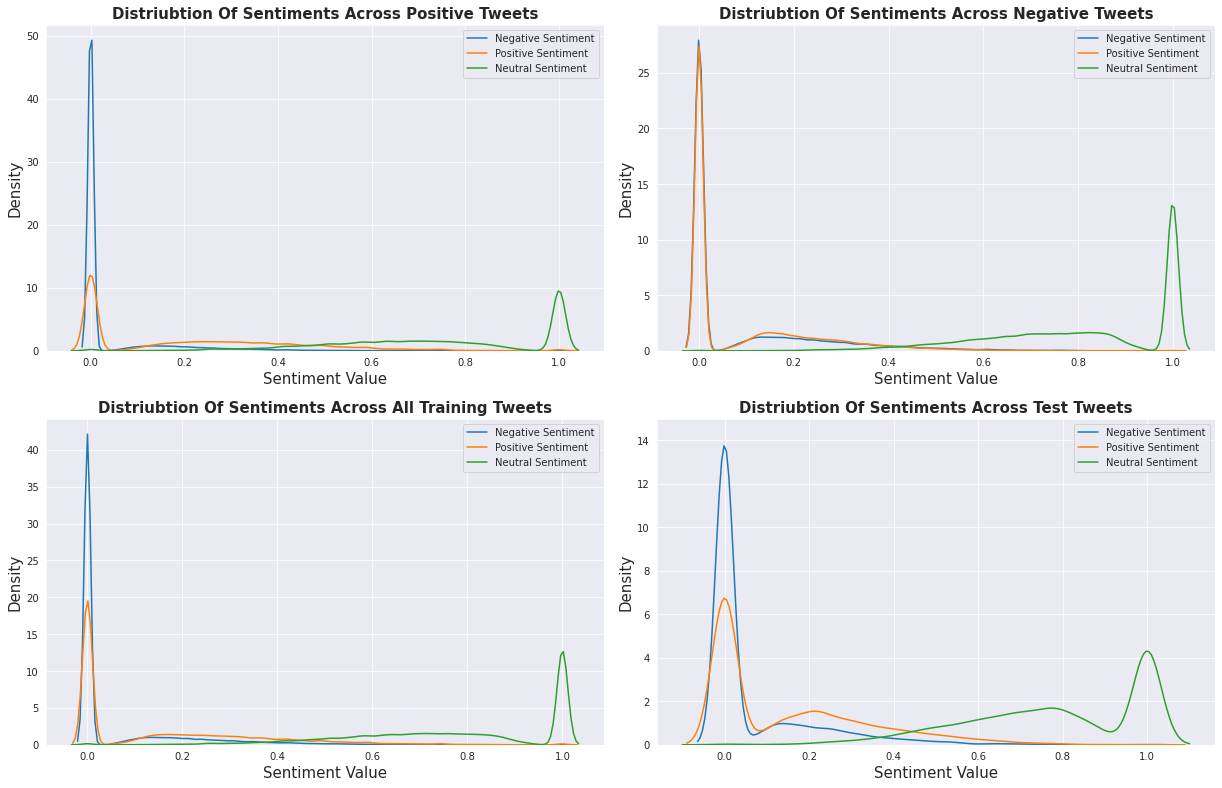
\includegraphics[width=0.35\textwidth]{distributions.png}
    \caption{\label{fig:distributions}Distributions of Sentiment Scores}
\end{figure}

From the plots, we can see positive tweets generally have higher positive sentiment scores and lower negative sentiment scores than negative tweets. For whichever tweet dataset, the neutral sentiment scores are much higher than its positive and negative sentiment scores, which means it would be important to make use of these neutral words to predict sentiment, and methods based on word embedding may not achieve very high accuracy. What is more, we can see there exists a visible distribution difference between training tweets and test tweets. It accounts for the weird behavior of BERT and XLNET we will later mention (accuracy goes up on the validation set but goes down on the test set).

\section{Data Pre-processing}
In this section, we will describe all the pre-processing methods we have tried in our project. Some of the methods turn out to be beneficial for model training and prediction, while some are too aggressive and hurt more than it helps. The final decision of pre-processing methods was based on theoretical analysis and some careful control experiments (we didn't carry out a comprehensive ablation study due to limited computation resources).

\textbf{Remove Duplicates:} By examining the training data, we find there are roughly 10\% duplicated tweets. Duplicates also appear after other pre-processing steps. We choose to remove these duplicates to reduce redundancy.

\textbf{Process Emoticons:} Emoticons appear frequently in both training and test dataset. They are written with different symbols but carry very similar sentimental information. To emphasize those expressing positive or negative feelings, we built a dictionary mapping each emoticon to a unification symbol (either $<$fjoy$>$ or $<$fsad$>$).

\textbf{Remove Stop Words:} Stop words carry little sentimental information but are very often used in sentences. We choose to remove them when using some word embedding-based classification. But for large models like BERT and XLNET, we keep them because they more or less carry some structural information.

\textbf{Process Numbers:} Numbers appear in numerous different formats in context and it is not a good idea to treat 2 numbers (like 37927 and 53701) as different words. We group whichever number is larger than 9 into 4 different groups according to their magnitude. That is, mapping 2-bits number to $<$nsma$>$, 3-bits number to $<$nmed$>$, 4-bits number to $<$nlar$>$, 5-bits and larger number to $<$nhug$>$.

\textbf{Process Repetition of Letters:} Some Twitter users may use the repetition of letters as a way to stress a word. But we don't want to treat 'youuuuuu' and 'youuuu' differently. Luckily in correct English spelling, a letter never appears more than twice in continuity, so we can replace more than 2 continuous identical letters with just 2 the same letters (e.g. 'yessss' to 'yess').

\textbf{Process Abbreviation:} Abbreviations in English spelling don't change the sentimental meaning of a phrase but add to the number of word embedding we need to create. So we just remove them with the help of regular expressions.

\textbf{Remove Punctuation:} Like stop words, punctuation generally doesn't carry sentimental information, but does carry structural information. So we process them like what we do to stop words.

\textbf{Word Stemming and Lemmatization:} Word stemming and lemmatization reduce inflectional forms and sometimes derivationally related forms of a word to a common base form. However, stemmers are too aggressive and lemmatizers have only limited generalization ability. To achieve the best utility, we choose to use Krovetzstemmer\cite{Krovetz_github}, which is a combination of stemmer and lemmatizer, for our pre-processing.

\textbf{Remove Conflicts:} Again by examining training data, we see there exists about 1,900 conflicted tweets (which appear in both positive and negative datasets). We just remove these tweets.

Experiment with both raw data and pre-processed data with CNN model in section VIII shows that the pre-processed data can improve the performance of the model by 1.4 \%.

\section{Word Representation}
In order to represent a text consisting of multiple words as a meaningful vector, we first need to represent the words as some meaningful vectors. This chapter will introduce some representations of word vectors as well as ways to obtain them.

\textbf{Word2Vec}  This approach uses a data-driven approach to capture the correlation between different words by analyzing how often words occur together in context, assuming that each word vector is of length $\lvert D \rvert$ and that we have selected N words in the corpus for computation, then we end up with a dictionary of size $N \times |D|$.

Depending on the method of implementation, we can divide Word2Vec into two categories, skipgram and cbow, which are distinguished as follows:

\textit{1)Skipgram} Given a target word, predict the words that occur in the context of that target word.

\textit{2)Cbow} In contrast to the skipgram, given a context word, cbow predicts what the target word is that has this context

generally speaking, skipgram takes a longer time than Cbow when training, but the word vectors produced by skipgram will be more accurate, especially for rare words that occur less frequently

\textbf{GloVe} The difference between GloVe method and Word2Vec method is that Word2Vec is a prediction-based model while GloVe is Count-based, i.e. Glove is obtained by dimensionality reduction of the co-occurrence matrix of words. In our experiments we have used the following three methods to implement GloVE:

\textit{1)Pre-Trained Model} We used the vector representations of 1.19 million words obtained by training the GloVe model on 2 billion tweeted texts. The words in this cover the vast majority of the words we need.

\textit{2)Self-Trained Model} We trained the GloVe model on our own corpus, by setting the window size to 4.

\textit{3)Merged Model} Although the Self-trained Model is largely encompassed by the Pre-trained Model, there are still some words that are not present in the Pre-trained Model, so here we take a concatenation of the two lexicons and use the vectors from the Pre-trained Model for the overlap.

\textbf{WordPiece Embedding} One of the main implementations of WordPiece is called BPE (Byte-Pair Encoding). For example, the words "loved", "loving" and "loves". The BPE algorithm is able to split the above three words into "lov", "ed", "ing" and "es" , thus effectively reducing the number of words in the list. We have used this coding in the Bert model.

\section{Tweet Representation}
For the task of classifying whole texts, we are really concerned with representing a sentence as a vector rather than a word vector. We can broadly divide the methods into two types: aggregate methods and non-aggregate methods
\subsection{Non-Aggregate Methods}
\textbf{Bag of Words} This is the simplest and most intuitive way to represent text. Assume that the set of words is of size $\lvert N \rvert$ and there are $\lvert X \rvert$ documents, then we'll generate a spars matrix of size $\lvert X \rvert \times \lvert N \rvert$, each entry $A_{ij}$ represents word $j$ appears $A_{ij}$ times in document $j$. To better distinguish between the importance of different words, we could use the Tf-IDF method, multiplying each element of the matrix by an IDF factor. To obtain semantic information, we could decompose the matrix to obtain a representation of the documents on the latent semantic space.

\textbf{Represent texts word by word} Instead of computing the representation of text based on some aggregation function on words vectors, we can simply represent the text word by word, assume a text with $\lvert K \rvert$ words, then this text can be represented by a matrix of size $K \times D$, which D is the length of each word vector. Furthermore, we can add position embedding and segment embedding, to distinguish different positions in a sentence and different sentences.

\subsection{Aggregate Method}
\textbf{MIN/MEAN/MAX Aggregation} We can simply calculate the min/mean/max vectors of all the vectors of words contained in this text, and consider the result as the representation of the text, this computation is possible because all word vectors have the same length, we've tried all of these methods in our experiments.

\textbf{learnable aggregation} Instead of explicitly aggregating all word vectors via min/mean/max, we can you learnable kernel to aggregate all vectors, in our experiment, we implemented two means of learnable aggregation with different kernel shapes, one uses unsquared kernels that only aggregate inter-words values, the other one uses squared kernel which also aggregate inner-word values. Fig. \ref{different_kernel} below shows the difference between these two methods.

\begin{figure}[h]
    \centering
        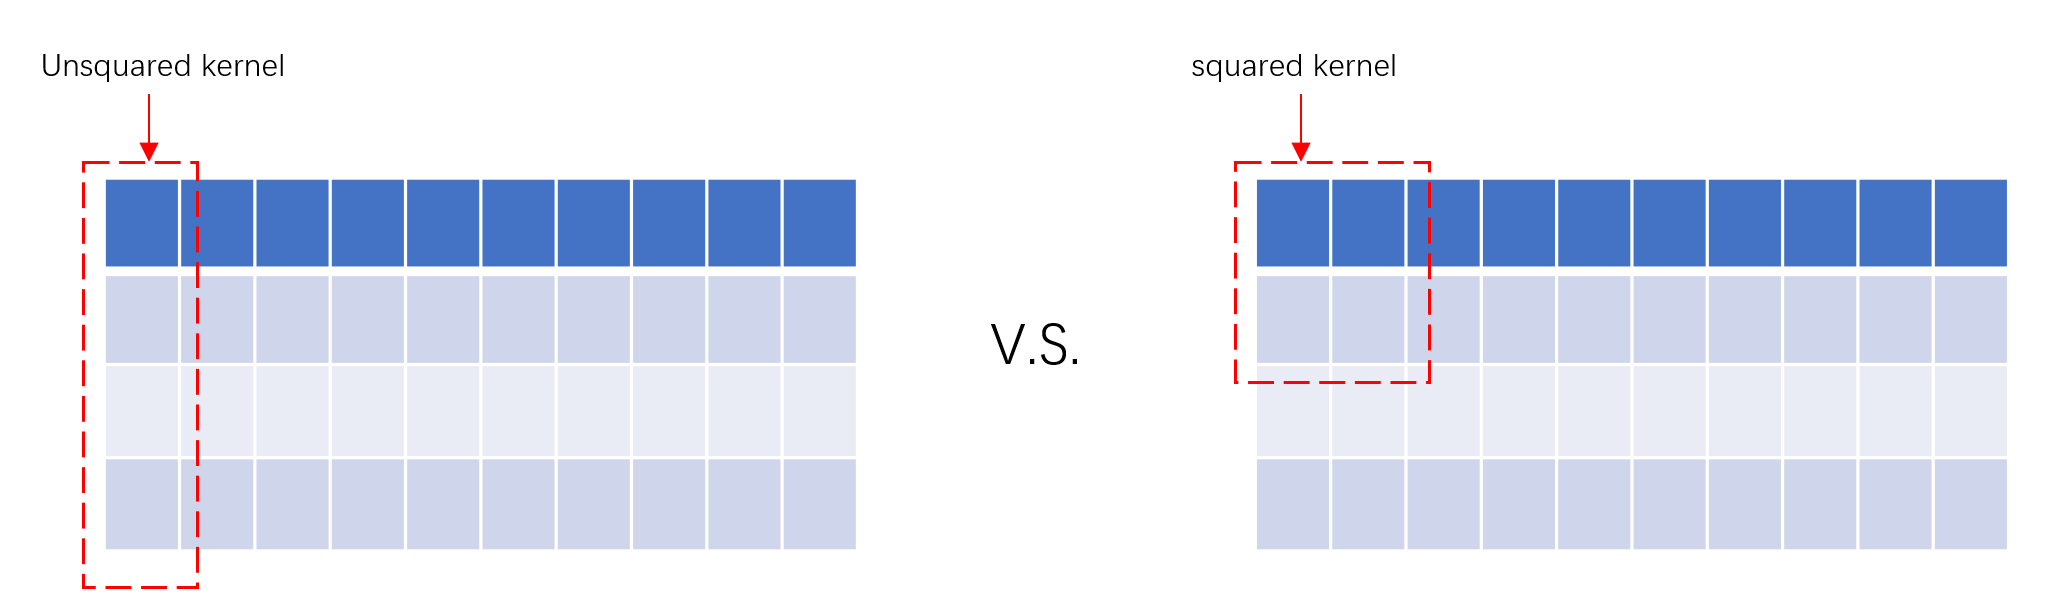
\includegraphics[width=0.35\textwidth]{different_kernel.png}
    \caption{\label{different_kernel}the different kernels we used to aggregate word vectors}
\end{figure}


\section{Classification}

\begin{figure}[h]
    \centering
        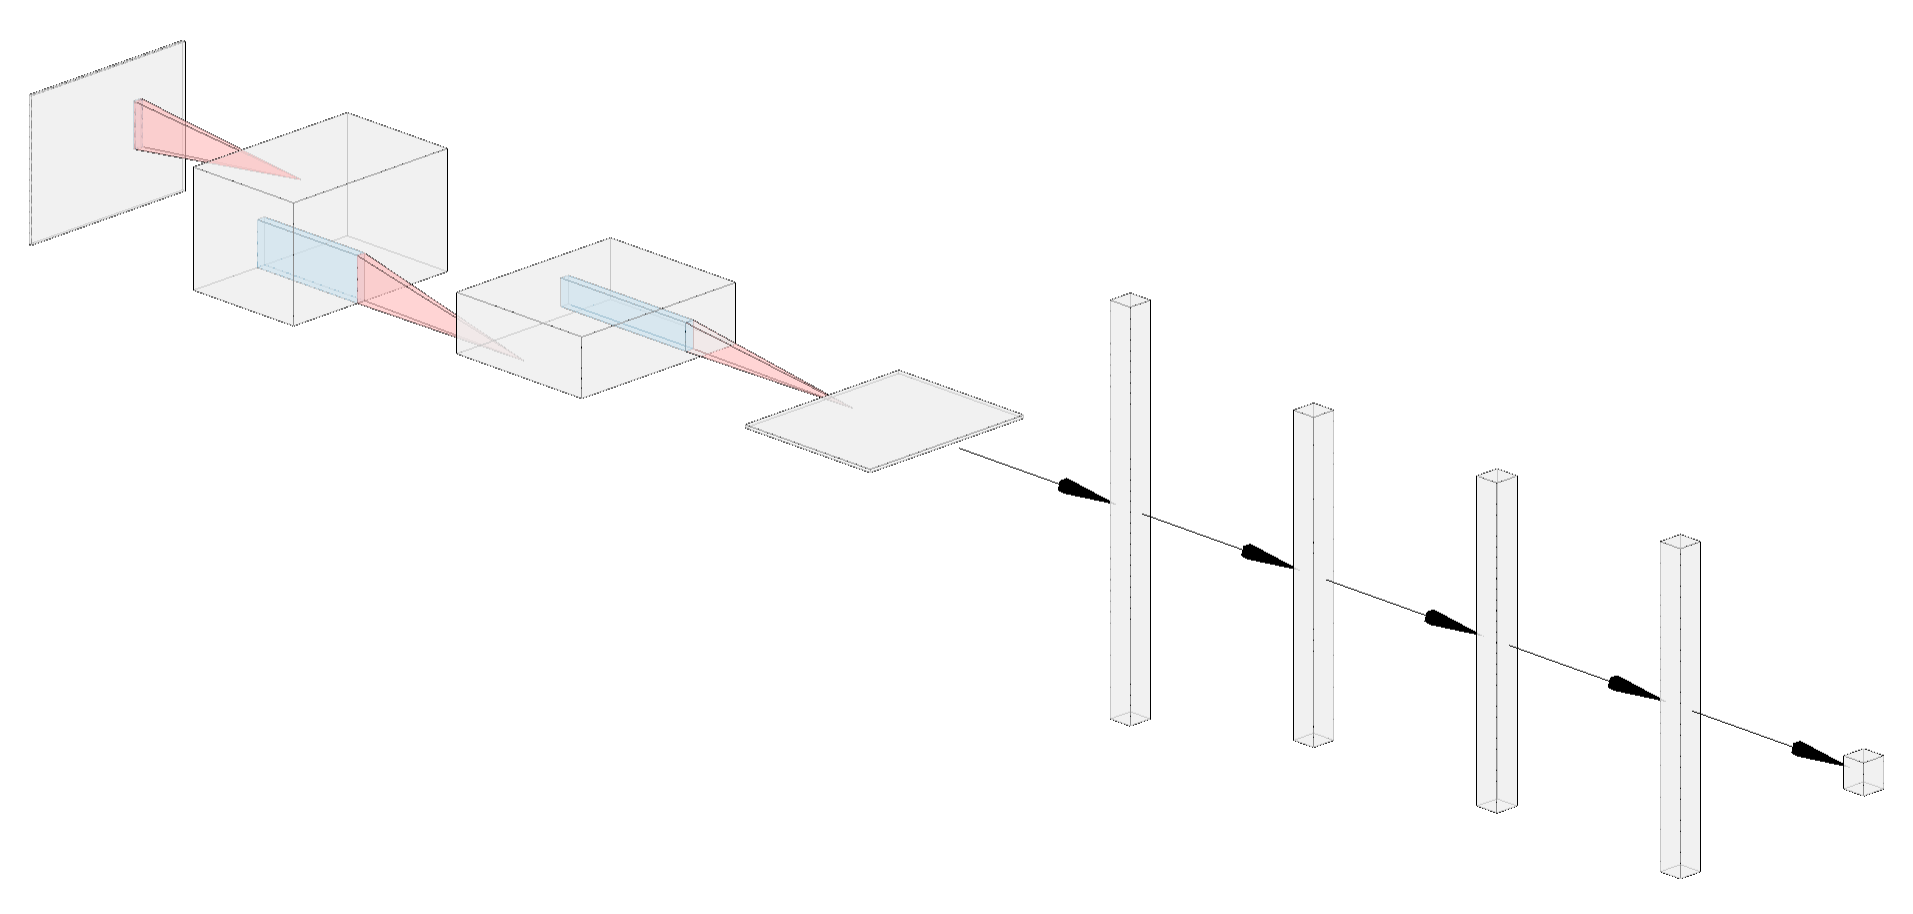
\includegraphics[width=0.35\textwidth]{cnn.png}
    \caption{\label{cnn}the CNN structure we implemented}
\end{figure}

\subsection{CNN}
For the final implementation of the CNN, we used a  relatively deep network that uses unsquared kernels, the structure of the network is shown in Fig. \ref{cnn}, we trained it for 50 epochs, and a decreasing learning rate with the initial value of 0.005, finally achieved 81.6\% accuracy on the test data.

\subsection{Transformer}
Transformer, based solely on attention mechanisms, dispensing with recurrence and convolutions entirely, is a model proposed by Google in 2017.\cite{transformer} We introduce Encoder structure in Transformer together with Glove embedding to this task and achieve an accuracy rate of 85\% in the test dataset.
\subsection{BERT}
In 2019, Google Brain Team proposed a new language representation model called BERT, which stands for Bidirectional Encoder Representations from Transformers.\cite{bert} BERT is designed to pre-train deep bidirectional representations from
unlabeled text by jointly conditioning on both
left and right context in all layers. 

BERT contains two parameter intensive settings.

\textbf{BERT-base}: The number of Transformer blocks is 12, the hidden layer size is 768, the number of self-attention heads is 12, and the total number of parameters for the pre-trained model is 110M.

\textbf{BERT-large}: The number of Transformer blocks is 24, the hidden layer size is 1024, the number of self-attention heads is 16, and the total number of parameters for the pre-trained model is 340M.

Restricted by hardware resources, we implement \textit{bert-base-uncased} as our pre-trained model. In \cite{bert}, the author illustrates that the pre-trained BERT model can be finetuned with an additional output layer
to create state-of-the-art models for a wide range of tasks, including sentiment analysis, without substantial task-specific architecture modifications. Therefore, along with BERT, we add a 2-layer fully connected classifier with one non-linear function between them as our output layer to help classify data sentiment. Then, we use the Twitter dataset to do fine-tuning. All hyper-parameters are shown on the table.
\bigskip
\begin{center}
\begin{tabular}{ccc}
\hline
Hyper-parameter Name& Value\\
\hline
Classifier Layer 1& Linear(768,50) \\
Classifier Non-linear Func& ReLU \\
Classifier Layer 2& Linear(50,2) \\
BERT Token Length&  128\\
Learning Rate&  2e-5\\
Batch Size&  32\\
Epoch&  4\\
\hline
\end{tabular}
\end{center}
With this model, we can achieve an accuracy rate of 89.7\%. It is worth mentioning that using the BERT output vector's first token to predict directly without an additional classifier will result in an accuracy rate of 86.4\%, 3.3\% lower than the classifier implemented.
\subsection{BERTweet}
BERTweet is the first public largescale pre-trained language model for English Tweets.\cite{bertweet} BERTweet, having the same architecture as BERT, is
trained using the RoBERTa pre-training procedure. Because our dataset is collected in English Tweets, we believe a pre-trained model in Tweets will provide better behavior. We choose \textit{vinai/bertweet-base} as our pre-trained model with the same classifier in BERT Section. All other hyper-parameters also stay the same.
\begin{figure}[H]
\centering
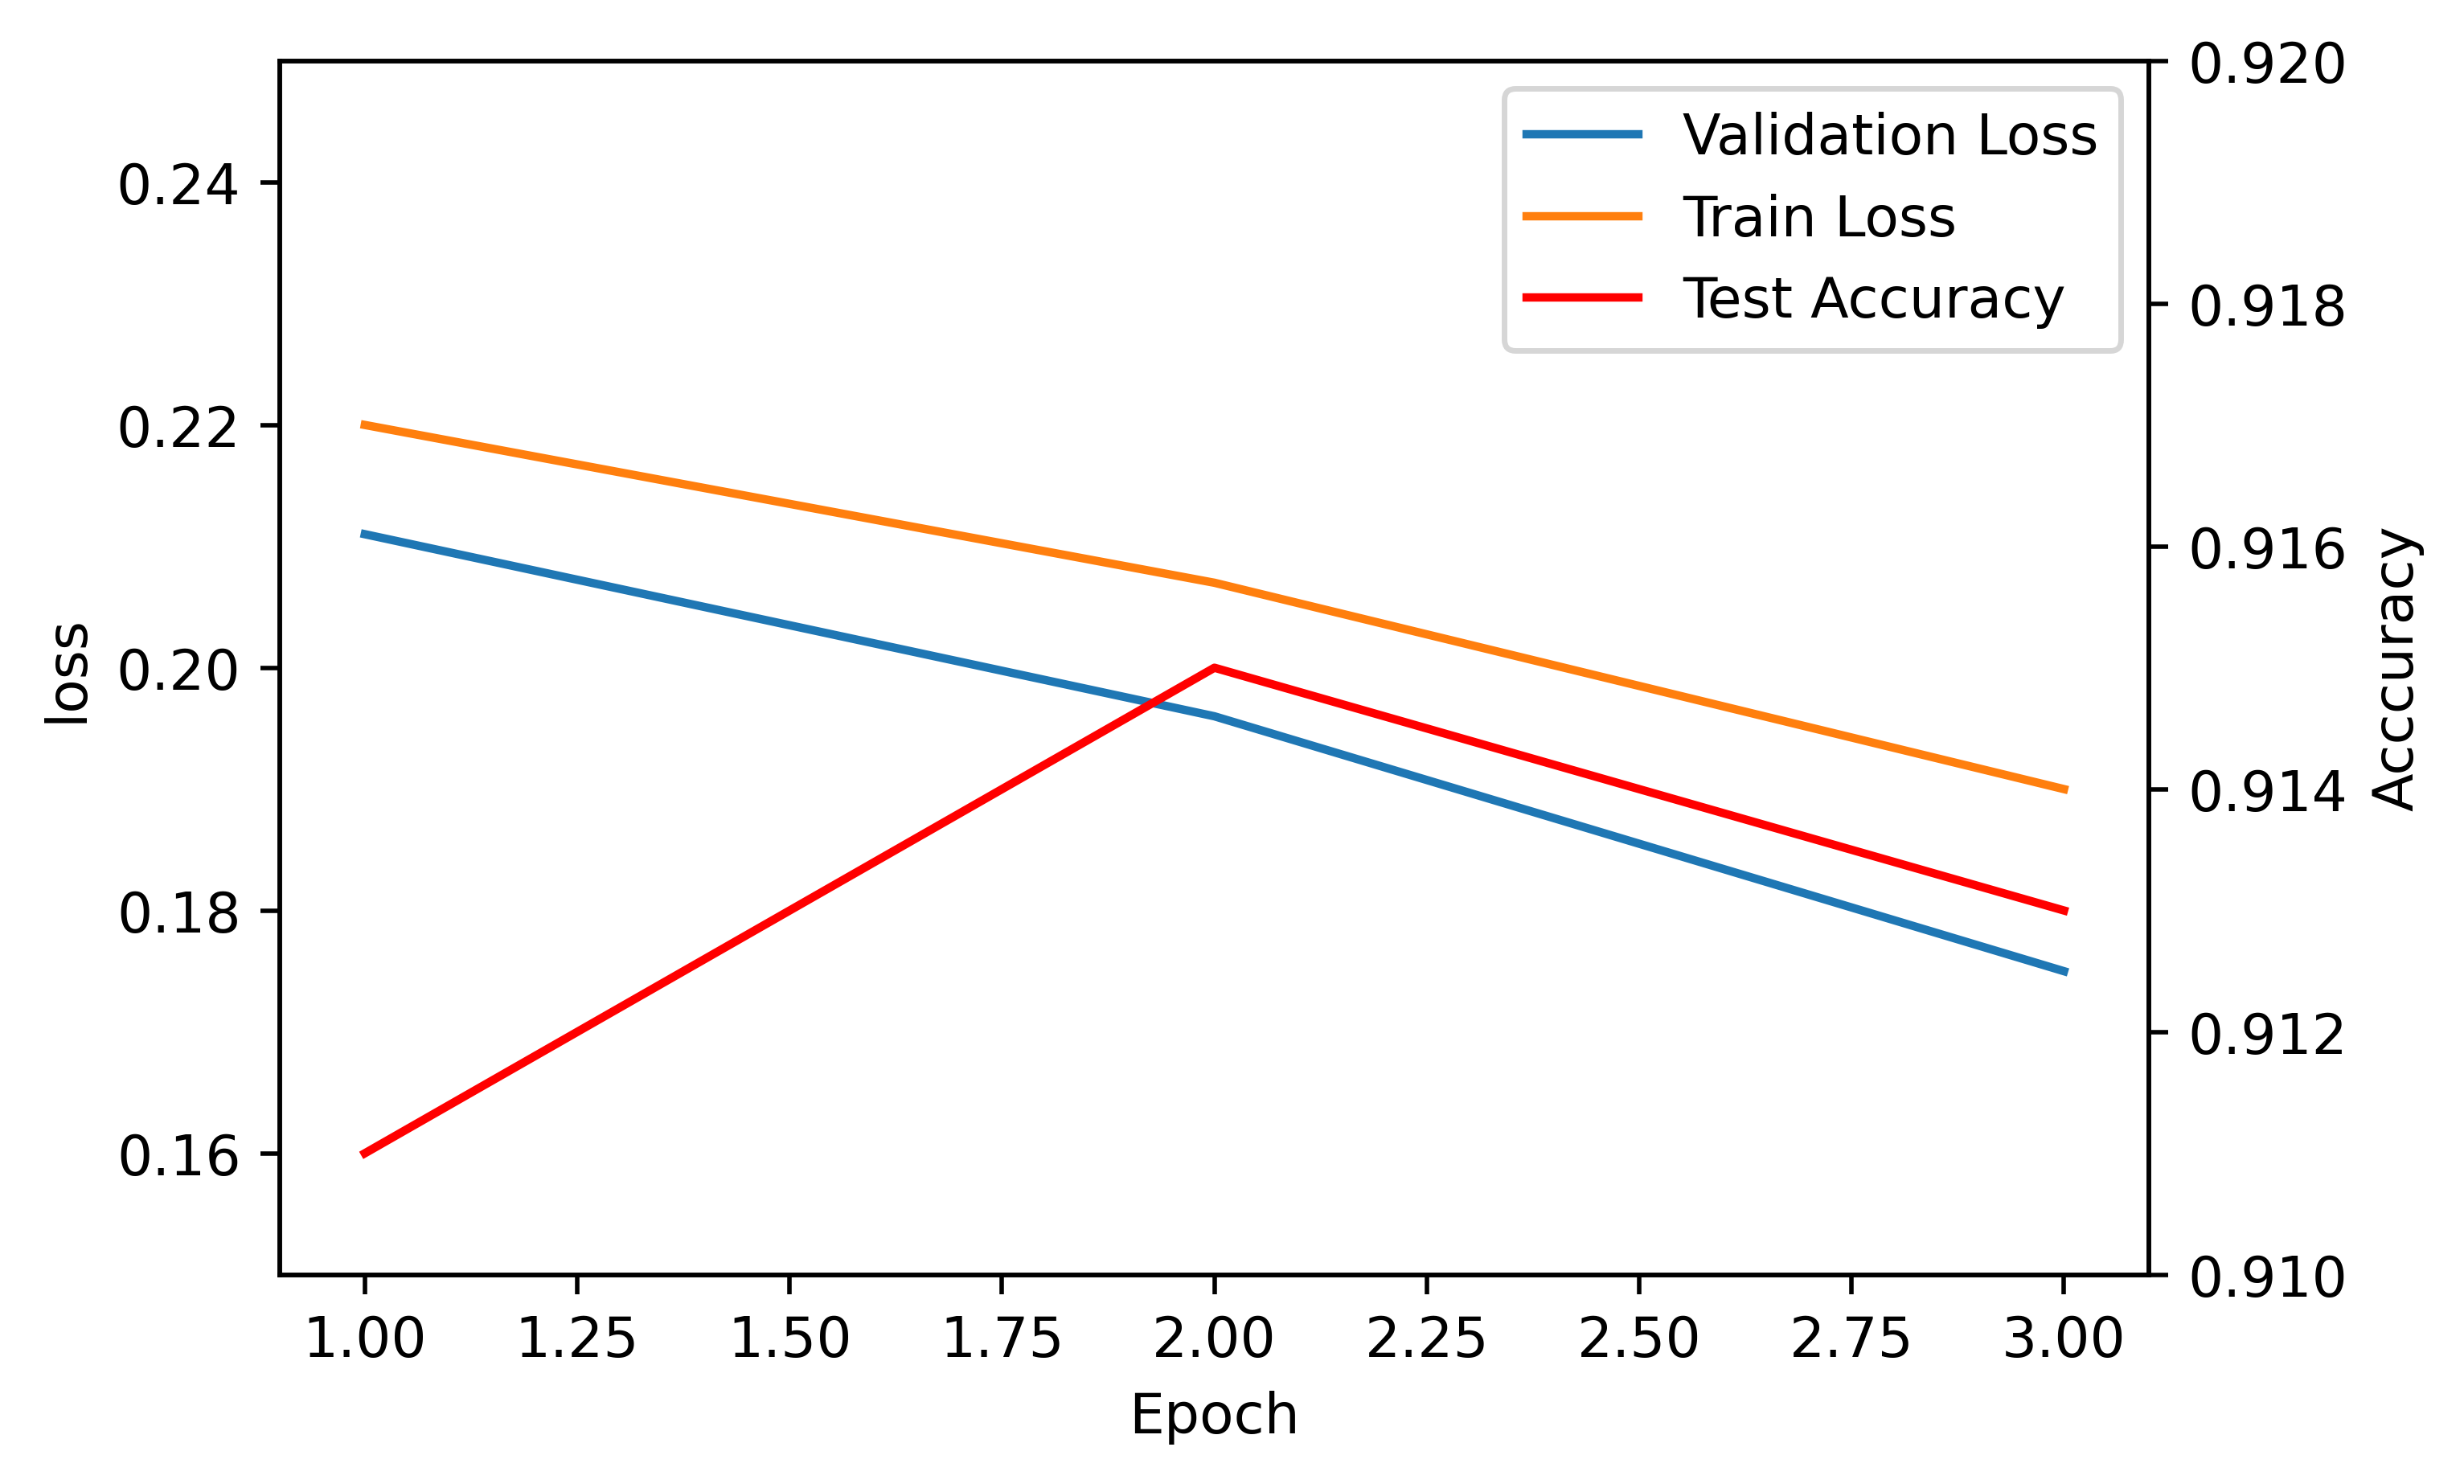
\includegraphics[width=0.35\textwidth]{bertweet.png}
\caption{Train and Validation Loss, Test Accuracy with Epoch}
\label{bertweet}
\end{figure}
Experiment results are shown in Fig. \ref{bertweet}. It points out that BERTweet with 2 epochs fine-tuning has the best result in test data, with an accuracy rate of 91.5\%, which is the second-highest accuracy rate in Aicrowd.
The training loss and validation loss are always dropping in training progress. After the third epoch, validation accuracy achieves more than 93\% while the model is still not over-fitted and has the potential to achieve higher. However, as shown in the Data Analysis section, the test data distribution and train data distribution are not the same, resulting in inconsistent test accuracy and validation accuracy.

\subsection{XLNet}
XLNet\cite{xlnet} is an extension of the Transformer-XL model proposed by Zhilin Yang et al. in 2019. It is pre-trained using an autoregressive method to learn bidirectional contexts by maximizing the expected likelihood over all permutations of the input sequence factorization order.

XLNet is included in python Transformers library so we can easily finetune it with a pre-trained model. For the single sequence classification problem we deal with, input tweets need to be converted to the form of 'seq $<$sep$>$ $<$cls$>$' to be fed into the model. Besides, XLNet accepts only fixed-length input, the tokenized tweets which are not long enough need to be padded to their pre-defined maximum length (64 or 128 in our experiments).

For the best result, XLNet can achieve an accuracy of 89.8\% on AIcrowd with $lr = 2e-5$, $max\_length = 64$ and 2 epochs of training on pre-processed dataset. The validation accuracy keeps growing while the test accuracy decreases after the third epoch, which is probably because of the distribution difference between training set and test set, as is shown in Data Analysis.

\section{Conclusion}
All our experiment results are shown in this table.

\begin{center}
    \begin{tabular}{c c}
    \hline
    Implement Method Name& Test Accuracy\\
    \hline
    CNN+unsquared kernel+deep network& 81.6\%\\
    fasttext+N-grams=4& 83.7\%\\
    Glove-Merged+Mean+SVM=4& 82.3\%\\
    BERT&  86.4\%\\
    BERT + Classifier&  89.7\%\\
    \textbf{BERTweet + Classifier}&  \textbf{91.5\%}\\
    XLNet& 89.8\%\\
    \hline
    \end{tabular}
\end{center}
This table points out that large-scale models tend to have better performance than other methods. It is very reasonable because large-scale models are the latest ones and have much higher computation complexity. Among all different methods, BERTweet shows the best test accuracy and ranks 2nd in Aicrowd.


\section{Ablation Study} We conducted several experiments to choose different important parameters and methods, Because of the large computational resources required to test on large scale models, this section focuses on smaller scale models.
\begin{figure}[h]
    \centering
        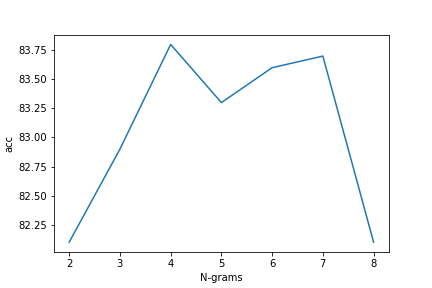
\includegraphics[width=0.35\textwidth]{N-grams.png}
    \caption{\label{N-grams}The accuracy when choosing different N-grams values}
\end{figure}
\subsection{N-grams selection} 
We use the supervised method provided by fasttext to try different N-grams values and see which of them perform the best. Here we set the training epochs to 50 and the dimension of word vectors to 200. As shown in Fig. \ref{N-grams}, the model achieves the best performance when N-grams equals 4.

\begin{figure}[h]
    \centering
        \includegraphics[width=0.35\textwidth]{aggregate_method.png}
    \caption{\label{aggregate}the accuracy when choosing different Word2Vec methods and aggregate methods}
\end{figure}

\subsection{Word2Vec methods selection}
We conducted our experiment on this part with SVM classifier and fasttext. According to Fig. \ref{aggregate}, skipgram performs better than cbow on all aggregation methods, which testify the assumption of the last chapter, although it takes longer to train a word embedding via skipgram method, Its multiple predictions for each central word in a single training session lead to higher quality training results.

\subsection{aggregate methods selection}
According to Fig. \ref{aggregate}, the Mean value performs better than the other two, which means in order to better classify the sentiment of a text, we need to take all words of the text into consideration.

\subsection{GloVe Methods selection}
We've implemented all three GloVe Methods with mean aggregation and SVM, 
We discovered that the Merged method has the best result:1.0\% better than the Pre-Trained model, 0.4\% better than the Self-Trained model. This is because it takes advantage of both the larger dataset and more comprehensive training of the Pre-Trained model, and also complements the missing words in the Pre-trained model with the Self-trained model. 

\subsection{CNN structure selection}
When choosing the structure of CNN, we conducted multiple experiments. Following table is the experimental data:

\bigskip
\begin{center}
\begin{tabular}{|l|r|}
\hline 
Method&Accuracy\\
\hline  
squared+shallow&78.2\\
\hline 
squared+deep&78.5\\
\hline
unsquared+shallow&80.0\\
\hline
unsquared+deep&81.6\\
\hline
\end{tabular}
\end{center}

which is as expected, because the deep network performs better than the shallow one, and the unsquared kernel is better than the squared one since it makes more sense to aggregate values of different word vectors instead of aggregate values in the same word vector. Finally, we've conducted this experiment with both raw data and pre-processed data, we found that the pre-processed data can improve the performance of the model by 1.4 \%.


\begin{thebibliography}{99}  
\bibitem{nlp} Liddy, Elizabeth D. "Natural language processing.", 2nd edn. Encyclopedia of Library and Information Science, Marcel Decker, 2001.
\bibitem{Krovetz_github}Ruey-Cheng Chen, KrovetzStemmer, (2020), GitHub repository, https://github.com/rmit-ir/KrovetzStemmer.
\bibitem{transformer}{Vaswani, Ashish, et al. "Attention is all you need." Advances in neural information processing systems. 2017.}
\bibitem{bert}{Kenton, Jacob Devlin Ming-Wei Chang, and Lee Kristina Toutanova. "Bert: Pre-training of deep bidirectional transformers for language understanding." Proceedings of NAACL-HLT. 2019.}
\bibitem{bertweet}Nguyen, Dat Quoc, Thanh Vu, and Anh Tuan Nguyen. "BERTweet: A pre-trained language model for English Tweets." arXiv preprint arXiv:2005.10200 (2020).
\bibitem{xlnet}Yang Z, Dai Z, Yang Y, et al. Xlnet: Generalized autoregressive pretraining for language understanding[J]. Advances in neural information processing systems, 2019, 32.
\end{thebibliography}

\end{document}
